\documentclass[12pt, letterpaper]{article}
\usepackage[a4paper, margin=1in]{geometry}
\usepackage{graphicx}
\usepackage{float}
\graphicspath{{images/}}
\author{Joseph Yu}
\title{Lab 2: Alignment between Spiking Neural Networks and Artificial Neural Networks}
\begin{document}
\maketitle
\setcounter{section}{4}
\subsection{Symmetric analysis of linear regression from CNN to SNN}
We are interested in exploring if there is a linear relationship between the output of the second batch normalization layer from the CNN to the second batch normalization layer of the SNN and vice versa. This can help to indicate whether or not the outputs are aligned or if one network's activations are tuned to the other network. We do this by first constructing a dataset of the activations from the CNN and SNN for all $10,000$ test images in the cifar dataset. We then perform linear regression on the dataset to determine if there is a linear relationship between the two networks' activations. The results of the linear regression are shown in Figure \ref{fig:lin_reg_loss}.

\begin{figure}[H]
    \centering
    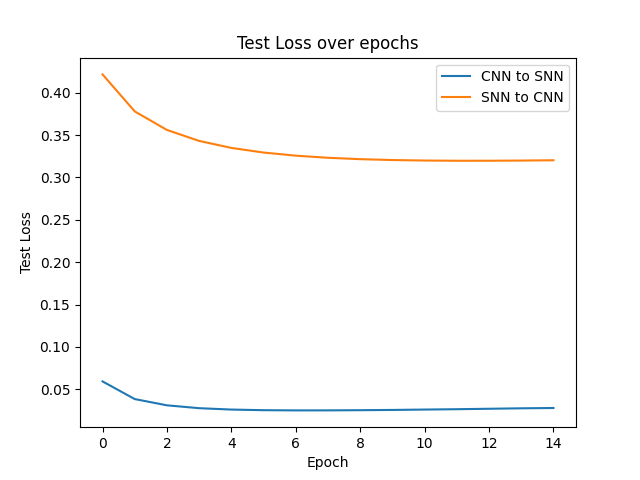
\includegraphics[width=0.75\textwidth]{lin_reg_loss.png}
    \caption{MSE loss of linear regression mapping from CNN to SNN and SNN to CNN}
    \label{fig:lin_reg_loss}
\end{figure}

We can see that there is a substantial difference in MSELoss between the two linear regressions. The MSELoss for the linear regression mapping from CNN to SNN is $0.025$ while the MSELoss for the linear regression mapping from SNN to CNN is around $0.33$. This suggest there is a linear mapping from CNN activations to SNN activations but not vice versa. One explanation is that visualizing the activations from the CNN and SNN as an image we can see that the CNN activations are more dense while the SNN activations are more sparse. In general mapping from a high dimensional space to a low dimensional space is easier than the reverse. This could be why the MSELoss for the CNN to SNN linear regression is lower than the SNN to CNN linear regression.

\begin{figure}[H]
    \centering
    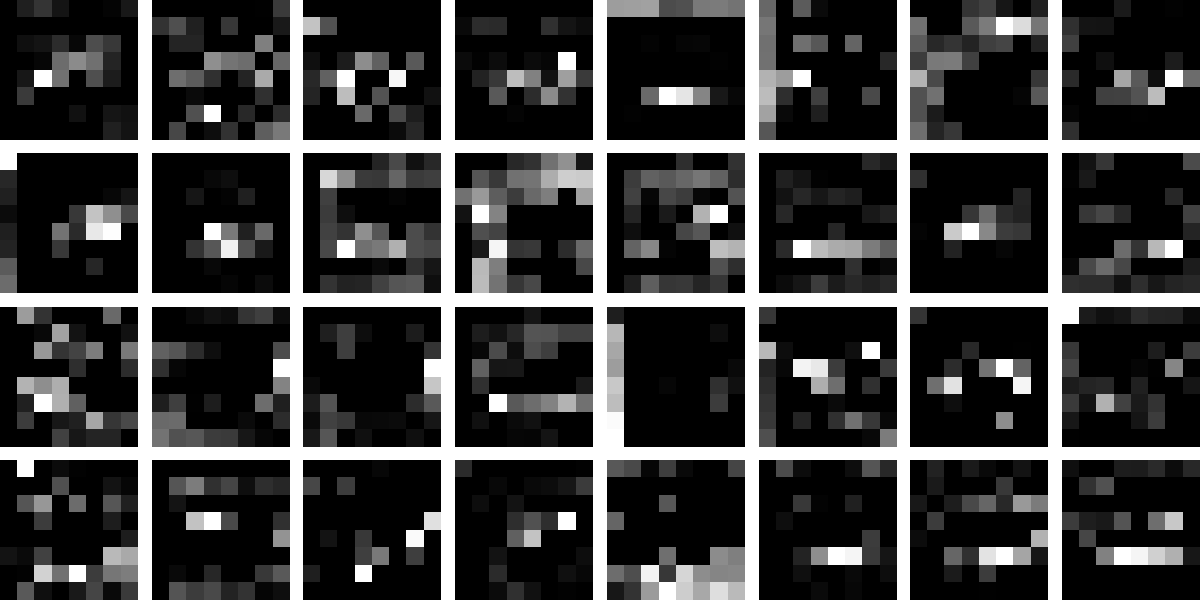
\includegraphics[width=0.75\textwidth]{conv2_cnn.png}
    \caption{Visual Representation for CNN 2nd BatchNorm Layer Activations}
    \label{fig:conv2_snn}
\end{figure}

\begin{figure}[H]
    \centering
    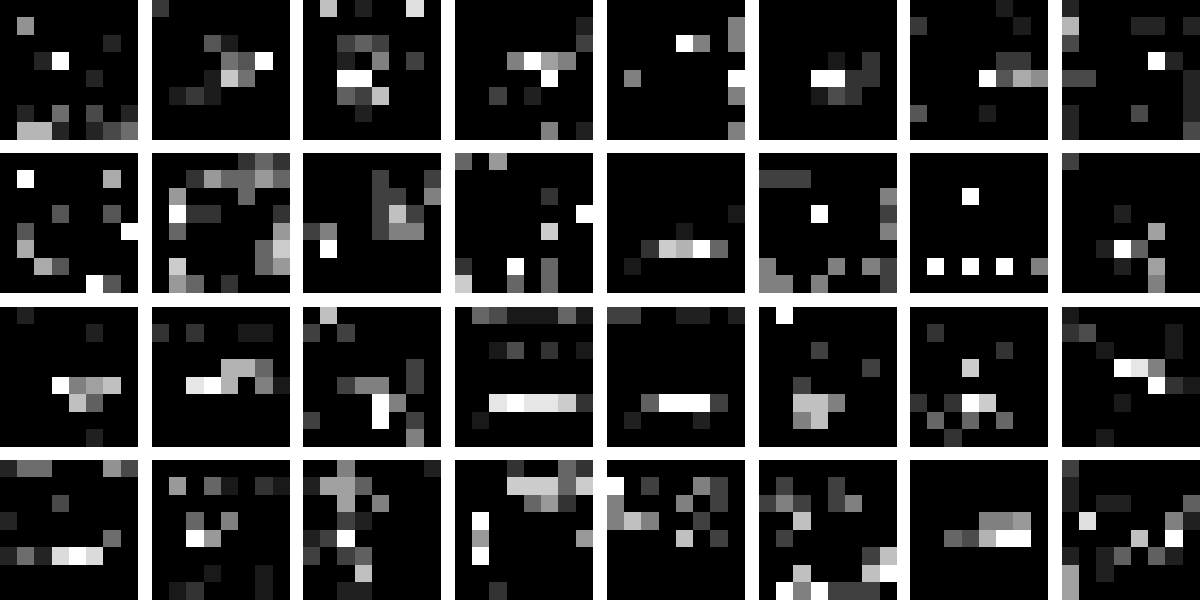
\includegraphics[width=0.75\textwidth]{conv2_snn.png}
    \caption{Visual Representation for SNN 2nd BatchNorm Layer Activations}
    \label{fig:snn_conv2}
\end{figure}

\subsection{Kernel visualization in AlexNet}
We are interested in visualizing the kernel weights for the first and second convolutional layers in a pretrained AlexNet model. The weights should help to indicate what the network is detecting in the input images that are helping the network to ultimately classify the images. 

\begin{figure}[H]
    \centering
    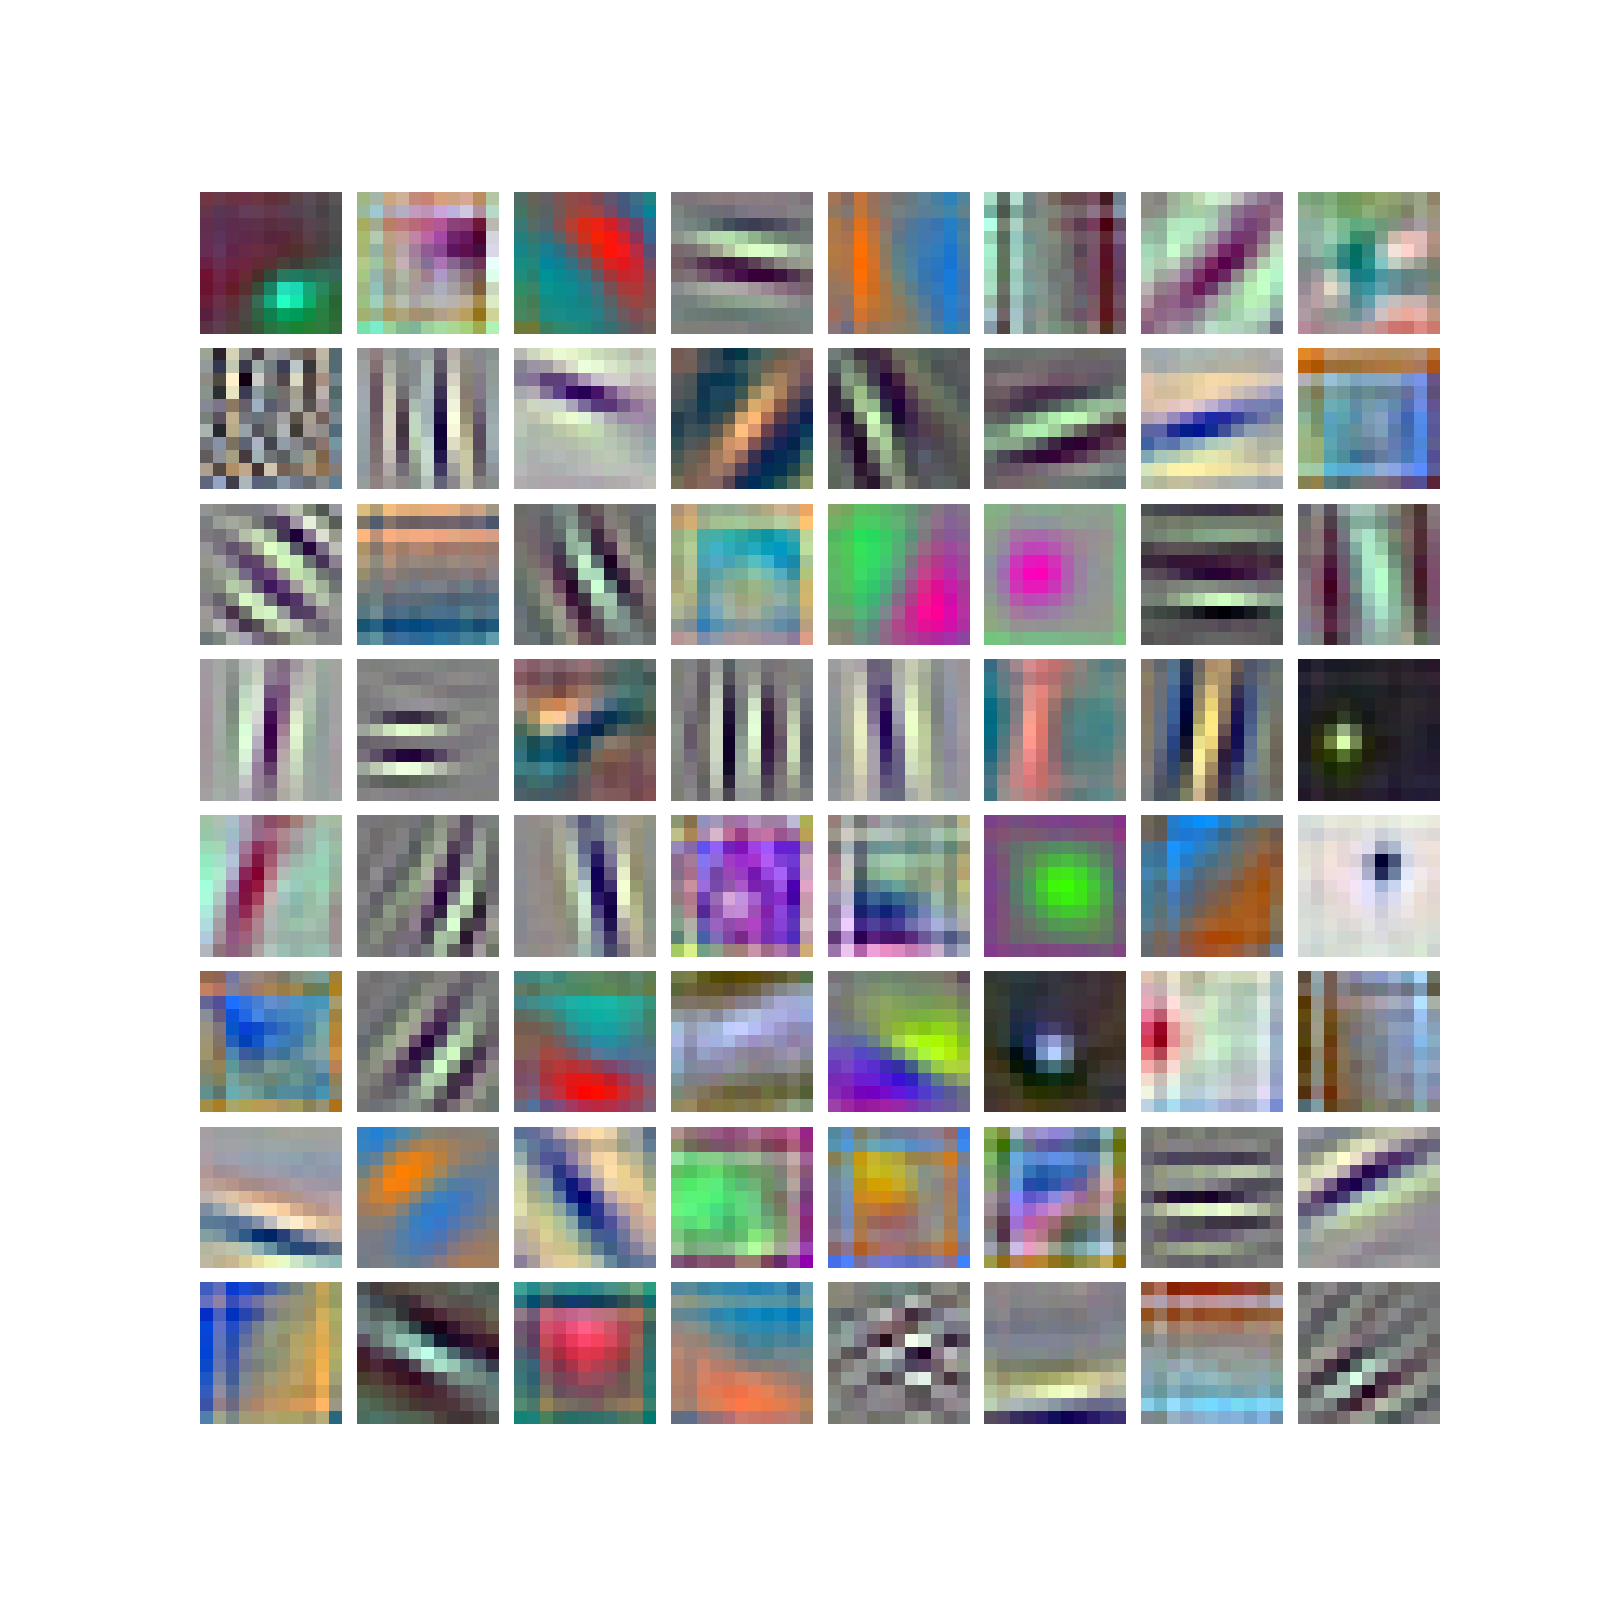
\includegraphics[width=0.75\textwidth]{alexnet_conv1.png}
    \caption{Visual Representation for AlexNet 1st Convolutional Layer Kernels}
    \label{fig:alexnet_conv1}
\end{figure}

The first convolutional layer has 64 kernels which are shown in Figure \ref{fig:alexnet_conv1}. We can see that the kernels are detecting edges and gradients in the input images. There are clear grating, checkboard, and gabor filter like patterns in the kernels. This is expected as the first convolutional layer is responsible for detecting low level features in the input images such as edges.

\begin{figure}[H]
    \centering
    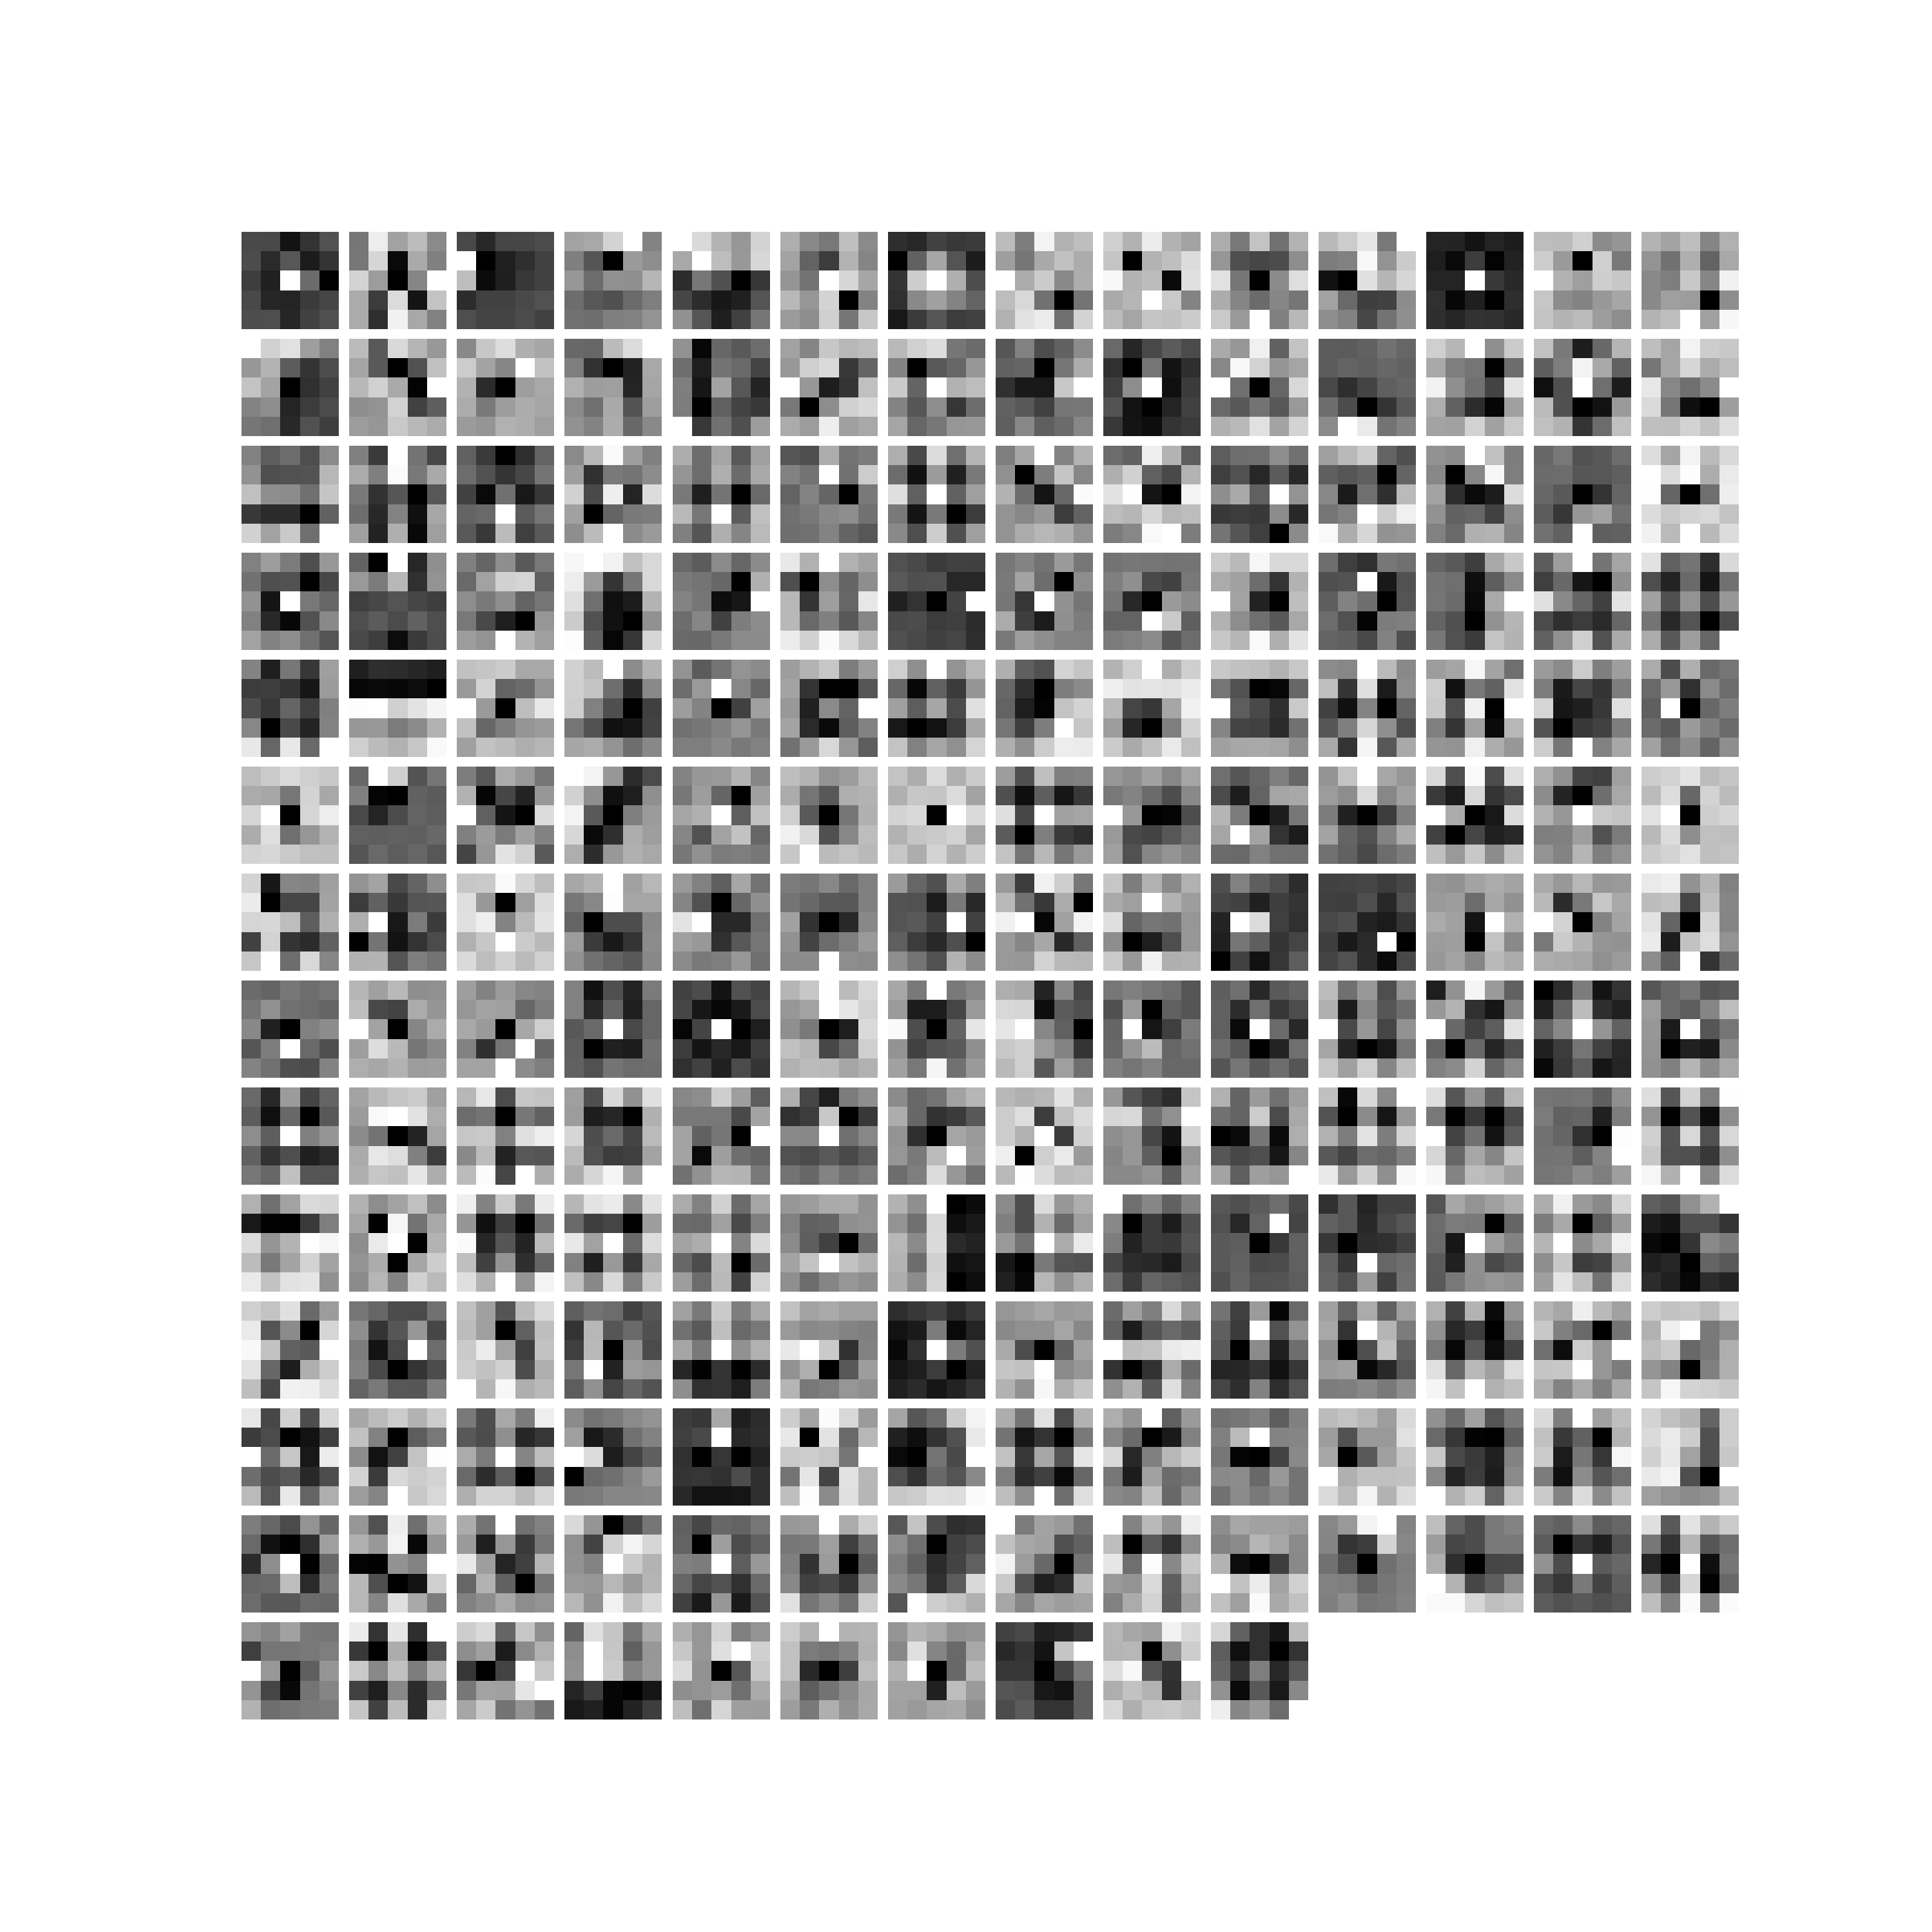
\includegraphics[width=0.75\textwidth]{alexnet_conv2.png}
    \caption{Visual Representation for AlexNet 2nd Convolutional Layer Kernels}
    \label{fig:alexnet_conv2}
\end{figure}

The second convolutional layer has 192 kernels which are shown in Figure \ref{fig:alexnet_conv2}. We can see that the kernels are detecting more complex patterns in the input images. Since the filters are smaller in size they are also more fine-grained compared to the first convolutional layer. From the visualization there are clear patterns of circles, squares, and other shapes. This result matches our expectations since similar to the ventral stream deeper layers are responsible for more complex feature detection.

\subsection{Feature Visualization in AlexNet}
Using activation maximization we can visualize the features that a particular layer, channel, or neuron is looking for using gradient descent. Starting with a noisey image we can keep the original AlexNet model parameters fixed and only update the input image to maximize the activation of a particular layer. 

\subsubsection{Visualize on a channel level}
We can specify a particular channel in a layer and visualize the features that the channel is looking for. 

\begin{figure}[H]
    \centering
    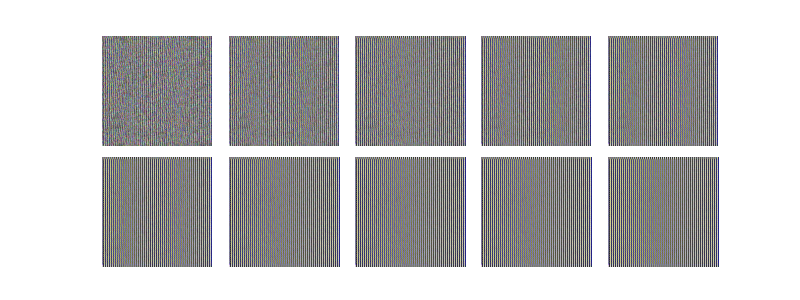
\includegraphics[width=1\textwidth]{alexnet_layer0_filter28.png}
    \caption{Visual Representation for AlexNet 1st Convolutional Layer Channel 28}
    \label{fig:alexnet_layer0_filter28}
\end{figure}

The visualization for the 28th channel in the first convolutional layer is shown in Figure \ref{fig:alexnet_layer0_filter28}. We can see that the image begins to develop a vertical grating pattern which is similar to the kernel weights in the first convolutional layer. This suggests that the 28th channel in the first convolutional layer is looking for vertical edges in the input images.

\subsubsection{Visualize on a neuron level}
We can specify a particular neuron using height and width coordinates within a channel in a layer and visualize the features that the neuron is looking for in its receptive field.

\begin{figure}[H]
    \centering
    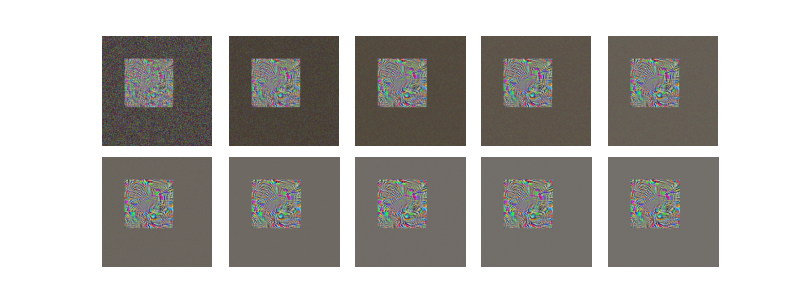
\includegraphics[width=1\textwidth]{alexnet_layer6_filter20_neuron5_5.png}
    \caption{Visual Representation for AlexNet 3rd Convolutional Layer Channel 20 Neuron 5, 5}
    \label{fig:alexnet_layer6_filter20_neuron5_5}
\end{figure}

The neuron visualization is interesting as we can see that the image has no distinct features except for within a small square region in the center. This suggests that the neuron is looking for a specific pattern in a specific region of the input image. The visual pattern is also more complex containing more circles and curves. 

\subsubsection{Visualize on a layer level}
We can also specify a particular layer and visualize the features that the entire layer is looking for.

\begin{figure}[H]
    \centering
    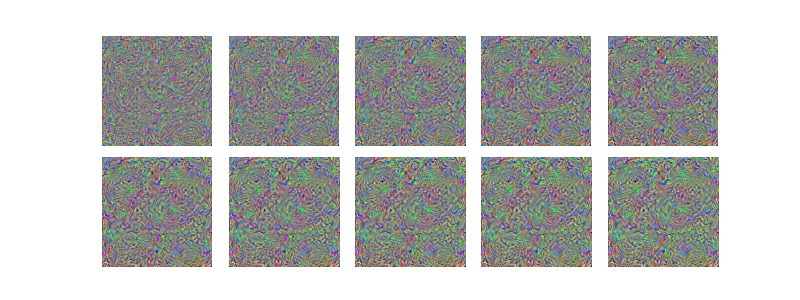
\includegraphics[width=1\textwidth]{alexnet_layer12.png}
    \caption{Visual Representation for AlexNet 5th Convolutional Layer}
    \label{fig:alexnet_layer12}
\end{figure}

The last convolutional layer visualization is much noisier compared to the channel and neuron visualizations. This is expected as the layer visualization is trying to maximize the activation of all the channels in the layer. The image is a mix of different complex patterns mostly circles, swirls, and curves. This also matches our expectations as the deeper layers in the network are responsible for detecting more complex features in the input images.

\subsection{Feature Visualization for SNN}

Since the activations in the SNN are discrete either the neuron fires or it doesn't we can't use activation maximization to visualize the features that a particular layer, channel, or neuron is looking for. Instead we can visualize the average of K input images that maximally activate a particular layer, channel or neuron in the SNN. For the following visualizations we set $K = 20$.

\begin{figure}[H]
    \centering
    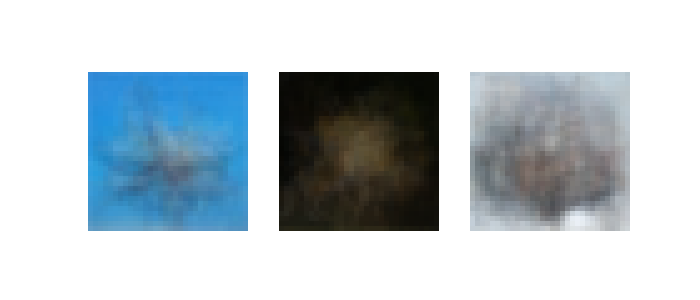
\includegraphics[width=1\textwidth]{snn_mean_images.png}
    \caption{Visual Representation for Mean Images that Maximally Activate SNN}
    \label{fig:snn_mean_images}
\end{figure}

From left to right we can see the mean images that maximally activate a particular layer, channel, or neuron in the SNN. We can see from the layer visualization that all the images have a solid blue background with wings/tendrils branching out of the center. In the channel visualization the mean image has a solid dark background with the central image being a light brown color. The central image has a spider/crab like shape. The neuron visualization is less intepretable with the mean iamge having a solid white background and some darker colors in the middle. One interesting observation is that for the neuron there is a clear white section in the bottom of the mean image. This could suggest that the neuron is looking for a specific pattern not in the center of the image but in the bottom.

\end{document}